\chapter{Testing, Reliability, dan Code Quality}
\label{ch:testing}

\section*{Tujuan Pembelajaran}
\begin{itemize}
  \item Membedakan unit test, integration test, dan End-to-End (E2E) test
        berdasarkan biaya waktunya dan jenis cacat yang tertangkap
        masing-masing.
  \item Merancang \textit{test double} dan pengujian kontrak untuk memisahkan
        bagian yang diuji dari layanan lain, lalu membuktikan pilihannya lewat
        pengujian yang berjalan tanpa layanan itu menyala.
  \item Mengukur mutu kode lewat \textit{coverage}, analisis statis, dan
        jumlah \textit{query} per alamat, lalu menegakkannya sebagai
        \textit{quality gate} yang memblokir \textit{merge}.
\end{itemize}

\section{Pendahuluan}

Bab 5 menutup pertanyaan tentang cepat atau lambat dengan angka. Yang belum
dijawab adalah pertanyaan yang lebih mendasar: apakah kodenya masih benar
sesudah diubah. Pada proyek kecil pertanyaan itu dijawab dengan mencoba
sendiri di browser. Cara itu berhenti bekerja begitu jumlah alamat bertambah,
karena tidak ada orang yang sanggup mencoba seluruhnya pada tiap perubahan.

Pengujian otomatis menggantikan percobaan tangan tersebut, tetapi tidak
seluruh pengujian sama harganya. Pengujian yang hanya menyentuh satu fungsi
selesai dalam milidetik, sedangkan pengujian yang membuka browser sungguhan
memakan detik. Keduanya menangkap cacat yang berbeda, dan salah satunya tidak
dapat menggantikan yang lain. Bab ini menyusun ketiganya sebagai satu
\textit{pipeline}, lalu memasang \textit{quality gate} yang membaca hasilnya
dan memblokir \textit{merge} yang cacat.

Seluruh angka pada bab ini diukur dari aplikasi pesanan di
\berkas{sources/chapter06/}. Referensi utamanya adalah dokumentasi pytest
\cite{pytest-docs} untuk kerangka pengujiannya, Playwright
\cite{playwright-docs} untuk lapisan E2E, Hypothesis
\cite{hypothesis-docs} untuk \textit{property-based testing}, serta uraian
piramida pengujian dari Cohn \cite{cohn2009succeeding} dan Fowler
\cite{fowler-pyramid} untuk menimbang jumlah tiap lapisan.

\section{Tiga Lapisan Pengujian}

Unit test menguji satu bagian kecil tanpa menyentuh apa pun di luarnya.
Integration test menguji beberapa bagian yang bekerja bersama, termasuk basis
data sungguhan. E2E test menjalankan aplikasinya seperti pengguna, lewat
browser, dan memeriksa apa yang tergambar di layar.

Analoginya seperti memeriksa sepeda sebelum dipakai. Memutar pedal di tempat
memeriksa satu bagian saja, murah dan cepat. Memasang rantai lalu memutarnya
memeriksa dua bagian sekaligus. Mengayuh sepedanya keliling lapangan
memeriksa seluruhnya, dan hanya cara terakhir yang membuktikan sepeda itu
benar-benar dapat dikendarai.

Tabel \ref{tab:lapisan} memuat pengukuran ketiga lapisan pada aplikasi bab
ini.

\begin{table}[!htb]
  \centering
  \caption{Waktu jalan tiap lapisan pengujian, hasil pengukuran nyata pada
           aplikasi Bab 6}
  \label{tab:lapisan}
  \begin{tabularx}{\textwidth}{lrrX}
    \hline
    \textbf{Lapisan} & \textbf{Jumlah} & \textbf{Waktu} & \textbf{Yang tertangkap} \\
    \hline
    Unit & 19 & 0,99 s & Salah hitung, salah batas, salah syarat \\
    \hline
    Integrasi dan kontrak & 15 & 1,27 s & Salah \textit{query}, bentuk \textit{response} berubah \\
    \hline
    E2E lewat Chrome & 5 & 2,90 s & Tombol tak terhubung, modul gagal dimuat \\
    \hline
  \end{tabularx}
\end{table}

Selisihnya jelas: satu pengujian E2E rata-rata memakan 0,58 detik, sekitar
sebelas kali lipat rata-rata satu unit test yang hanya 0,05 detik. Karena
harganya berbeda, jumlah tiap lapisan pun tidak dibuat sama.

Satu angka pada tabel tersebut perlu dibaca dengan hati-hati. Waktu E2E
bergoyang jauh lebih lebar daripada lapisan lain: tiga kali jalan berurutan
di komputer yang sama memberi 2,1 detik, 2,9 detik, dan 5,6 detik. Sebabnya
lapisan itu menyalakan browser sungguhan, dan browser ikut berebut prosesor
dengan apa pun yang sedang berjalan. Karena itu lapisan E2E tidak layak
dipakai sebagai pengukur waktu, dan pada \textit{gate} nanti yang dinilai
adalah lapisan unit dan integrasi. Gambar \ref{fig:piramida} memperlihatkan dua cara menyusun
perbandingannya.

\begin{figure}[!htb]
  \centering
  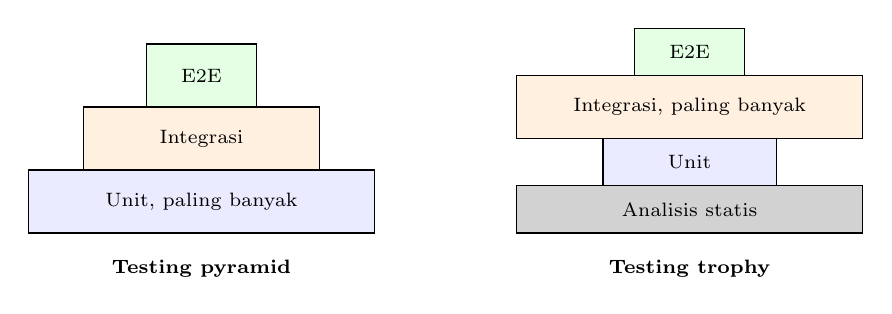
\begin{tikzpicture}[font=\scriptsize]
    % Piramida pengujian
    \fill[blue!8, draw=black] (0,0) rectangle (4.4,0.8);
    \node at (2.2,0.4) {Unit, paling banyak};
    \fill[orange!12, draw=black] (0.7,0.8) rectangle (3.7,1.6);
    \node at (2.2,1.2) {Integrasi};
    \fill[green!10, draw=black] (1.5,1.6) rectangle (2.9,2.4);
    \node at (2.2,2.0) {E2E};
    \node[font=\scriptsize\bfseries] at (2.2,-0.45) {Testing pyramid};

    % Testing trophy
    \fill[gray!35, draw=black] (6.2,0) rectangle (10.6,0.6);
    \node at (8.4,0.3) {Analisis statis};
    \fill[blue!8, draw=black] (7.3,0.6) rectangle (9.5,1.2);
    \node at (8.4,0.9) {Unit};
    \fill[orange!12, draw=black] (6.2,1.2) rectangle (10.6,2.0);
    \node at (8.4,1.6) {Integrasi, paling banyak};
    \fill[green!10, draw=black] (7.7,2.0) rectangle (9.1,2.6);
    \node at (8.4,2.3) {E2E};
    \node[font=\scriptsize\bfseries] at (8.4,-0.45) {Testing trophy};
  \end{tikzpicture}
  \caption{Piramida menekankan jumlah unit test, sedangkan \textit{trophy}
           memindahkan beratnya ke integration test dan menambahkan analisis
           statis sebagai alasnya}
  \label{fig:piramida}
\end{figure}

Dua bentuk pada gambar tersebut sering dipertentangkan, padahal keduanya
menjawab keadaan yang berbeda. Piramida \cite{cohn2009succeeding} lahir
ketika integration test masih mahal dan rapuh. \textit{Testing trophy}
\cite{dodds-trophy} lahir sesudah container membuat basis data sungguhan
dapat dinyalakan dalam hitungan detik, sehingga integration test menjadi
murah, dan analisis statis dapat menangkap sebagian cacat sebelum satu
pengujian pun berjalan.

\section{Test Double}

\textit{Test double} adalah pengganti sebuah bagian sungguhan saat pengujian
berjalan. Namanya diambil dari \textit{stunt double} di film: pemeran
pengganti yang dipakai pada adegan yang tidak perlu dikerjakan pemeran
aslinya.

Aplikasi bab ini memanggil layanan biaya kirim milik pihak lain lewat HTTP.
Memanggil layanan itu sungguhan membuat pengujiannya lambat, bergantung pada
jaringan, dan tidak dapat dijalankan ketika layanan tersebut sedang
\textit{down}. Tabel \ref{tab:double} memuat empat jenis penggantinya beserta
pertanyaan yang dijawab masing-masing.

\begin{table}[!htb]
  \centering
  \caption{Empat jenis \textit{test double} dan pertanyaan yang dijawabnya}
  \label{tab:double}
  \begin{tabularx}{\textwidth}{lXl}
    \hline
    \textbf{Jenis} & \textbf{Menjawab pertanyaan} & \textbf{Di Bab 6} \\
    \hline
    Dummy & Tidak menjawab apa pun, hanya mengisi argumen yang wajib ada & \texttt{Mock()} kosong \\
    \hline
    Stub & Apa hasilnya bila layanan menjawab nilai tertentu & \texttt{StubBiayaKirim} \\
    \hline
    Fake & Apakah aturannya benar untuk banyak masukan sekaligus & \texttt{FakeBiayaKirim} \\
    \hline
    Mock & Apakah layanannya dipanggil, dan dengan argumen apa & \texttt{Mock()} beserta \texttt{assert} \\
    \hline
  \end{tabularx}
\end{table}

Listing \ref{lst:double} memperlihatkan pemakaian mock untuk membuktikan
sesuatu yang tidak dapat dibuktikan dari nilai kembaliannya, yaitu bahwa
layanan luar tidak dipanggil sama sekali pada pesanan yang bebas ongkir.

\begin{lstlisting}[style=PythonStyle, caption={Mock membuktikan panggilan yang tidak terjadi, tersedia di \berkas{sources/chapter06/test\_double.py}}, label={lst:double}]
def test_mock_membuktikan_layanan_tidak_dipanggil():
  """Pesanan bebas ongkir tidak boleh memanggil layanan luar sama sekali.

  Sifat ini hanya dapat dibuktikan dengan mock, karena yang diperiksa bukan
  hasil hitungannya, melainkan ada atau tidaknya panggilan.
  """
  mock_klien = Mock()
  ongkir = layanan_kirim.hitung_ongkir(mock_klien, KODE_POS_JAKARTA,
                                       BERAT_GRAM, gratis_ongkir=True)
  assert ongkir == 0
  mock_klien.minta_biaya.assert_not_called()
\end{lstlisting}

Pertanyaan berikutnya, kapan penggantinya dipakai dan kapan tidak. Aturannya
satu kalimat: bagian yang dimiliki sendiri diuji apa adanya, sedangkan bagian
milik orang lain diganti. Basis data pada bab ini tidak diganti, karena
perilakunya justru yang ingin dibuktikan.

\section{Pengujian dengan Basis Data di Container}

Integration test pada bab ini memakai PostgreSQL sungguhan di dalam
container, bukan tiruan. Alasannya, cacat yang paling sering lolos justru
lahir dari perbedaan antara tiruan dan basis data aslinya, misalnya tipe
\texttt{numeric} yang tidak dikenal \texttt{json}, atau urutan baris yang
berbeda ketika \texttt{ORDER BY} lupa ditulis.

Masalahnya satu: pengujian yang menulis ke basis data akan mengotori data
uji, sehingga pengujian berikutnya bergantung pada urutan. Listing
\ref{lst:rollback} memperlihatkan jawabannya, yaitu membungkus tiap pengujian
di dalam transaksi yang selalu dibatalkan.

\begin{lstlisting}[style=PythonStyle, caption={Fixture yang mengembalikan basis data ke keadaan semula, tersedia di \berkas{sources/chapter06/conftest.py}}, label={lst:rollback}]
@pytest.fixture()
def koneksi():
  """Memberi satu koneksi basis data yang dibatalkan sesudah pengujian.

  Rollback membuat pengujian dapat menulis tanpa mengotori data uji, sehingga
  urutan pengujian tidak lagi menentukan hasilnya.
  """
  with basis_data.buka_koneksi() as koneksi_uji:
    yield koneksi_uji
    koneksi_uji.rollback()
\end{lstlisting}

Tabel \ref{tab:container} membandingkan kedua pilihan beserta waktu
menyiapkannya, diukur dari container yang belum menyala.

\begin{table}[!htb]
  \centering
  \caption{Tiruan basis data lawan PostgreSQL di container, waktu penyiapan
           hasil pengukuran nyata}
  \label{tab:container}
  \begin{tabularx}{\textwidth}{lXr}
    \hline
    \textbf{Pilihan} & \textbf{Akibatnya} & \textbf{Waktu siap} \\
    \hline
    Tiruan di memori & Cepat, tetapi tipe dan urutan barisnya tidak sama dengan aslinya & di bawah 0,1 s \\
    \hline
    Container, data sudah ada & Perilakunya persis basis data sungguhan & 0,9 s \\
    \hline
    Container, data diisi ulang & Sama, ditambah pengisian 50.000 baris data uji & 31,6 s \\
    \hline
  \end{tabularx}
\end{table}

Baris terakhir yang membuat orang ragu memakai container, padahal pengisian
data hanya dilakukan sekali. Sesudah datanya ada, container yang sudah
menyala siap dipakai dalam 0,9 detik, dan itulah yang dialami tiap kali
pengujian dijalankan.

Aturan ini punya dua konsekuensi praktis. Pertama, pengujian boleh ditulis
dalam urutan apa pun dan tetap memberi hasil yang sama. Kedua, data uji tidak
perlu dibangun ulang antarpengujian, sehingga 15 pengujian integrasi dan
kontrak selesai dalam 1,27 detik.

\section{Pengujian API dan Contract Testing}

Pengujian kontrak memeriksa bentuk \textit{response}, bukan isinya. Yang
dijaga adalah janji yang dipegang klien: nama field, tipenya, dan field mana
yang selalu ada. Janji itu ditulis sebagai JSON Schema
\cite{jsonschema-2020} di \berkas{sources/chapter06/kontrak/pesanan.schema.json},
lalu dipakai pengujian untuk memeriksa server.

Bedanya dengan integration test terasa ketika sebuah field ditambahkan.
Integration test tetap hijau, karena nilai yang diperiksanya tidak berubah.
Pengujian kontrak justru menyala, karena skemanya menutup field tambahan
lewat \texttt{additionalProperties} bernilai \texttt{false}. Tabel
\ref{tab:kontrak} memuat apa saja yang diperiksa.

\begin{table}[!htb]
  \centering
  \caption{Pemeriksaan pada pengujian kontrak alamat pesanan}
  \label{tab:kontrak}
  \begin{tabularx}{\textwidth}{lX}
    \hline
    \textbf{Yang diperiksa} & \textbf{Janjinya} \\
    \hline
    Status 200 & Bentuk \textit{response} cocok dengan skema, tanpa field tambahan \\
    \hline
    Tipe field & \texttt{id} dan \texttt{total} bilangan bulat, \texttt{status} salah satu dari empat nilai \\
    \hline
    Status 400 & Id bukan angka ditolak tanpa menyentuh basis data \\
    \hline
    Status 404 & Id yang tidak ada dijawab 404, bukan 500 \\
    \hline
    Header & \texttt{X-Query-Count} selalu ada dan berisi angka \\
    \hline
  \end{tabularx}
\end{table}

\section{Property-Based Testing}

Unit test biasa menyebutkan contoh satu per satu, dan hanya memeriksa contoh
yang terpikirkan penulisnya. \textit{Property-based testing} membalik
urutannya: yang ditulis adalah sifat yang harus selalu benar, lalu pustakanya
yang mencari angka pembantahnya \cite{hypothesis-docs}.

Listing \ref{lst:properti} memperlihatkan satu sifat pada aturan harga.
Ketika tanda bandingnya salah, Hypothesis menemukan contoh tepat di batas dan
menyusutkannya menjadi contoh terkecil yang masih gagal.

\begin{lstlisting}[style=PythonStyle, caption={Sifat yang harus selalu benar, bukan contoh satu per satu, tersedia di \berkas{sources/chapter06/test\_properti.py}}, label={lst:properti}]
@given(jumlah_unit=UNIT, harga_satuan=HARGA_SATUAN)
def test_diskon_tidak_melebihi_subtotal(jumlah_unit, harga_satuan):
  """Potongan selalu lebih kecil daripada belanjanya, sehingga tidak gratis."""
  subtotal = harga.hitung_subtotal(jumlah_unit, harga_satuan)
  assert 0 <= harga.hitung_diskon(jumlah_unit, subtotal) <= subtotal
\end{lstlisting}

Tabel \ref{tab:properti} memuat keempat sifat yang diuji beserta biayanya.
Tiap sifat dicoba dengan seratus contoh, yaitu bawaan Hypothesis, sehingga
empat sifat berarti empat ratus contoh dalam satu kali jalan.

\begin{table}[!htb]
  \centering
  \caption{Empat sifat yang diuji, masing-masing dengan seratus contoh, hasil
           pengukuran nyata}
  \label{tab:properti}
  \begin{tabularx}{\textwidth}{Xl}
    \hline
    \textbf{Sifat yang dijaga} & \textbf{Contoh} \\
    \hline
    Total tidak pernah negatif & 100 \\
    \hline
    Potongan tidak melebihi belanjanya & 100 \\
    \hline
    Menambah unit tidak menurunkan subtotal & 100 \\
    \hline
    Pesanan grosir selalu mendapat potongan & 100 \\
    \hline
    Empat sifat, satu kali jalan & 400 contoh dalam 0,9 s \\
    \hline
  \end{tabularx}
\end{table}

Empat ratus contoh dalam 0,9 detik itu yang membuat lapisan ini layak
dijalankan sesering unit test biasa, walaupun jumlah pengujiannya hanya
empat.

\section{Analisis Statis dan Batas Coverage}

Analisis statis membaca kode tanpa menjalankannya, lalu melaporkan hal yang
mencurigakan: nama yang tidak pernah dipakai, \textit{import} yang menggantung,
atau perbandingan yang selalu benar. Pada bab ini alatnya \texttt{ruff}
\cite{ruff-docs}, dan hasilnya nol temuan pada seluruh file sumber.

\textit{Coverage} mengukur berapa banyak baris yang tersentuh saat pengujian
berjalan. Angkanya mudah dibaca, dan justru karena itu mudah dipercaya
berlebihan. Tabel \ref{tab:coverage} memperlihatkan sebabnya.

\begin{table}[!htb]
  \centering
  \caption{Coverage \berkas{harga.py} dengan dan tanpa pengujian batas, 23
           pernyataan, hasil pengukuran nyata}
  \label{tab:coverage}
  \begin{tabularx}{\textwidth}{Xrr}
    \hline
    \textbf{Suite yang dijalankan} & \textbf{Pengujian} & \textbf{Coverage} \\
    \hline
    Seluruh \berkas{test\_harga.py} & 10 & 100\% \\
    \hline
    Tanpa pengujian batas, \texttt{-k "not batas\_grosir"} & 9 & 100\% \\
    \hline
  \end{tabularx}
\end{table}

Kedua suite menyentuh seluruh baris, sehingga angkanya sama-sama 100 persen.
Perbedaannya baru terlihat ketika kodenya dirusak dengan sengaja. Percobaan
itu disebut \textit{mutation testing}: satu tanda banding diubah, lalu
pengujiannya dijalankan ulang. Tabel \ref{tab:mutasi} memuat hasilnya untuk
mutasi \texttt{>=} menjadi \texttt{>} pada \texttt{hitung\_diskon}.

\begin{table}[!htb]
  \centering
  \caption{Hasil mutasi \texttt{>=} menjadi \texttt{>} pada
           \texttt{hitung\_diskon}, hasil pengukuran nyata}
  \label{tab:mutasi}
  \begin{tabularx}{\textwidth}{Xll}
    \hline
    \textbf{Suite yang dijalankan} & \textbf{Coverage} & \textbf{Hasil} \\
    \hline
    Tanpa pengujian batas & 100\% & 9 lolos, mutasi tidak tertangkap \\
    \hline
    Seluruh pengujian & 100\% & 1 gagal, mutasi tertangkap \\
    \hline
  \end{tabularx}
\end{table}

Angka itu menjelaskan batas \textit{coverage} dalam satu kalimat:
\textit{coverage} menjawab baris mana yang dijalankan, bukan apakah hasilnya
diperiksa. Pesanan tepat sepuluh unit adalah satu-satunya contoh yang
membedakan kedua tanda banding, dan contoh itulah yang hilang pada suite
pertama.

\section{Quality Gate di CI}

Seluruh pengukuran di atas baru berguna bila ada yang menegakkannya pada tiap
perubahan. Gambar \ref{fig:gate-mutu} memperlihatkan tempatnya bekerja.

\begin{figure}[!htb]
  \centering
  \begin{tikzpicture}[
    font=\scriptsize,
    kotak/.style={draw, rounded corners, minimum height=0.9cm, minimum width=2.1cm,
                  align=center, font=\scriptsize\bfseries},
    panah/.style={-{Stealth[length=2mm]}, thick}
  ]
    \node[kotak, fill=blue!8] (ubah) at (0,0) {Perubahan\\kode};
    \node[kotak, fill=blue!8] (uji) at (3.0,0) {Jalankan uji\\{\tiny\mdseries pytest, Playwright}};
    \node[kotak, fill=orange!12] (nilai) at (6.2,0) {Nilai mutu\\{\tiny\mdseries mutu.json}};
    \node[kotak, fill=green!10] (gabung) at (9.6,0.9) {Status 0\\{\tiny\mdseries boleh digabung}};
    \node[kotak, fill=red!22] (tolak) at (9.6,-0.9) {Status 1\\{\tiny\mdseries merge diblokir}};

    \draw[panah] (ubah) -- (uji);
    \draw[panah] (uji) -- (nilai);
    \draw[panah] (nilai.east) -- ++(0.5,0) |- (gabung.west);
    \draw[panah] (nilai.east) -- ++(0.5,0) |- (tolak.west);
    \node[font=\tiny, gray, anchor=east] at (7.7,0.72) {seluruh batas terpenuhi};
    \node[font=\tiny, gray, anchor=east] at (7.7,-0.72) {ada batas dilanggar};
  \end{tikzpicture}
  \caption{Mutu dinilai pada tiap perubahan, dan \textit{verdict}-nya dibaca
           \textit{Continuous Integration} sebagai status keluar}
  \label{fig:gate-mutu}
\end{figure}

Batasnya ditulis di satu file, \berkas{sources/chapter06/mutu.json}, dan
diperlakukan seperti kode. Isinya empat jenis: batas waktu tiap lapisan
pengujian, \textit{coverage} minimum, jumlah temuan analisis statis yang
ditoleransi, dan jumlah \textit{query} maksimum tiap alamat. Listing
\ref{lst:gate-mutu} memperlihatkan penutup gerbangnya, dan Listing
\ref{lst:gate-mutu-jalan} memuat keluarannya apa adanya.

\begin{lstlisting}[style=PythonStyle, caption={Status keluar yang memblokir merge, tersedia di \berkas{sources/chapter06/gate-mutu.py}}, label={lst:gate-mutu}]
  jumlah_langgar = sum(1 for baris in daftar_baris if not baris[-1])
  if jumlah_langgar:
    print(f"\nGagal: {jumlah_langgar} batas mutu dilanggar.")
    sys.exit(1)
  print("\nLolos: seluruh batas mutu terpenuhi.")
\end{lstlisting}

\begin{lstlisting}[language=bash, caption={Menjalankan gate mutu, tersedia di \berkas{sources/chapter06/gate-mutu.py}}, label={lst:gate-mutu-jalan}]
source ../.venv/bin/activate
python gate-mutu.py
echo $?

# Keluarannya:
#   Pemeriksaan                             Batas            Terukur  Verdict
#   pytest unit                                 0                 0   lolos
#   waktu unit                                 10 s           1.89 s  lolos
#   pytest integrasi                            0                 0   lolos
#   waktu integrasi                            30 s           2.12 s  lolos
#   coverage harga.py                          95 %            100 %  lolos
#   temuan ruff                                 0                 0   lolos
#   query /api/pesanan/1                        2                 2   lolos
#   query /api/pesanan-n1/1                     2                 5   LANGGAR
#
# Gagal: 1 batas mutu dilanggar.
# 1
\end{lstlisting}

Baris terakhir keluaran itu yang paling penting. Alamat
\texttt{/api/pesanan-n1/1} memberi \textit{response} yang sama persis dengan
alamat sehat, dan seluruh pengujian isinya hijau. Yang membedakannya hanya
jumlah \textit{query}, yaitu 5 lawan 2 untuk pesanan berisi tiga item. Cacat
seperti itu tidak terbaca dari \textit{response}, dan hanya tertangkap karena
jumlahnya ikut diukur.

\section{Ringkasan}

Pengujian otomatis bukan satu benda, melainkan tiga lapisan dengan harga dan
hasil tangkapan yang berbeda. Sembilan belas unit test selesai dalam 0,99
detik, lima belas pengujian integrasi dan kontrak dalam 1,27 detik, sedangkan
lima pengujian E2E lewat Chrome memakan 2,90 detik. Karena harganya berbeda,
jumlahnya pun tidak dibuat sama, dan itulah yang digambarkan piramida
pengujian maupun \textit{testing trophy}.

Bagian milik orang lain diganti saat pengujian, bagian milik sendiri diuji
apa adanya. Layanan biaya kirim diganti stub, fake, atau mock sesuai
pertanyaan yang ingin dijawab, sedangkan PostgreSQL tetap dipakai sungguhan
di dalam container. Tiap pengujian integrasi dibungkus transaksi yang selalu
dibatalkan, sehingga urutan pengujian berhenti menentukan hasilnya.

Bentuk \textit{response} dijaga terpisah dari isinya. Kontraknya ditulis
sebagai JSON Schema, dan pengujian kontrak memeriksa server terhadap file
itu. Menambah satu field yang tidak diumumkan akan lolos dari integration
test, tetapi tertangkap kontraknya.

\textit{Coverage} menjawab pertanyaan yang lebih sempit daripada yang sering
dikira. Dua suite yang berbeda sama-sama mencetak 100 persen pada
\berkas{harga.py}, tetapi hanya satu yang menangkap mutasi \texttt{>=}
menjadi \texttt{>}. Angka \textit{coverage} menyatakan baris mana yang
dijalankan, bukan apakah hasilnya benar-benar diperiksa.

Seluruhnya baru berarti ketika ada yang menegakkannya. Gerbang mutu membaca
\berkas{mutu.json}, menilai waktu tiap lapisan, \textit{coverage}, temuan
analisis statis, dan jumlah \textit{query} per alamat, lalu keluar dengan
status 1 begitu satu batas dilanggar. Pada aplikasi bab ini, satu-satunya
yang dilanggar adalah jumlah \textit{query} alamat N+1, yaitu cacat yang
tidak terlihat sama sekali dari \textit{response}-nya.

\section{Latihan}

Seluruh file yang dipakai pada latihan ini tersedia di
\berkas{sources/chapter06/}, dihitung relatif terhadap akar repositori.
Latihan membutuhkan Docker dengan Compose versi 2, Python 3, Node.js, dan
Google Chrome yang sudah terpasang. Listing penyiapan masuk ke direktori itu
lebih dahulu, dan seluruh perintah sesudahnya dijalankan dari sana.

Seluruh kegiatan pada bab ini hanya menyentuh basis data dan aplikasi milik
sendiri di komputer sendiri, sehingga tidak ada sistem pihak lain yang
dibebani. Hasil tiap mahasiswa akan berbeda, karena waktunya bergantung pada
perangkat keras dan beban lain yang sedang berjalan. Yang dilaporkan adalah
pola perbandingannya, bukan angka persisnya.

Penyiapannya dilakukan sekali, seperti pada Listing \ref{lst:c6-siapkan}.

\begin{lstlisting}[language=bash, caption={Menyiapkan basis data, data uji, dan dependensi, memakai \berkas{sources/chapter06/siapkan-data.sh}}, label={lst:c6-siapkan}]
cd sources/chapter06
docker compose up -d
./siapkan-data.sh
python3 -m venv ../.venv
../.venv/bin/pip install "psycopg[binary]" pytest hypothesis jsonschema \
  coverage ruff
npm install
\end{lstlisting}

\subsection*{Latihan 1: Membandingkan Tiga Lapisan Pengujian}

Latihan ini membuktikan bahwa ketiga lapisan berbeda harganya, dan menangkap
cacat yang berbeda pula.

\begin{enumerate}
  \item Jalankan ketiga lapisan seperti pada Listing
        \ref{lst:c6-lat1-jalan}, lalu catat jumlah pengujian dan waktunya ke
        Tabel \ref{tab:c6-lat1-hasil}. Tabel \ref{tab:c6-lat1-contoh}
        memperlihatkan contoh yang sudah terisi.
  \item Hitung berapa kali lipat satu pengujian E2E dibandingkan rata-rata
        satu unit test.
  \item Matikan aplikasinya, lalu jalankan ulang lapisan E2E dan catat apa
        yang terjadi. Nyalakan kembali sesudahnya.
  \item Jawab tiga pertanyaan berikut. Pertama, cacat apa yang hanya
        tertangkap lapisan E2E? Kedua, mengapa unit test tetap dibuat paling
        banyak walaupun paling sempit jangkauannya? Ketiga, apa akibatnya
        bila seluruh pengujian dipindahkan ke lapisan E2E?
\end{enumerate}

\begin{lstlisting}[language=bash, caption={Menjalankan ketiga lapisan pengujian, memakai \berkas{sources/chapter06/}}, label={lst:c6-lat1-jalan}]
source ../.venv/bin/activate
pytest -q test_harga.py test_properti.py test_double.py
pytest -q test_integrasi.py test_kontrak.py
python aplikasi.py &
npx playwright test --config e2e/playwright.config.ts
\end{lstlisting}

\begin{table}[!htb]
  \centering
  \caption{Contoh hasil Latihan 1 yang sudah terisi}
  \label{tab:c6-lat1-contoh}
  \begin{tabularx}{\textwidth}{lrrX}
    \hline
    \textbf{Lapisan} & \textbf{Jumlah} & \textbf{Waktu} & \textbf{Catatan} \\
    \hline
    Unit & 19 & 0,99 s & Tanpa basis data dan tanpa jaringan \\
    \hline
    Integrasi dan kontrak & 15 & 1,27 s & Basis data di container \\
    \hline
    E2E & 5 & 2,90 s & Chrome sungguhan, satu \textit{worker} \\
    \hline
  \end{tabularx}
\end{table}

\begin{table}[!htb]
  \centering
  \caption{Lembar isian hasil pengukuran Latihan 1}
  \label{tab:c6-lat1-hasil}
  \begin{tabularx}{\textwidth}{lrrX}
    \hline
    \textbf{Lapisan} & \textbf{Jumlah} & \textbf{Waktu} & \textbf{Catatan} \\
    \hline
    Unit & \dots & \dots & \dots \\
    \hline
    Integrasi dan kontrak & \dots & \dots & \dots \\
    \hline
    E2E & \dots & \dots & \dots \\
    \hline
    E2E tanpa aplikasi menyala & \dots & \dots & \dots \\
    \hline
  \end{tabularx}
\end{table}

\subsection*{Latihan 2: Coverage yang Menipu}

Latihan ini membuktikan bahwa \textit{coverage} 100 persen tidak menjamin
cacat tertangkap.

\begin{enumerate}
  \item Ukur \textit{coverage} \berkas{harga.py} untuk seluruh
        \berkas{test\_harga.py}, lalu ukur lagi tanpa pengujian batas,
        seperti pada Listing \ref{lst:c6-lat2-jalan}.
  \item Ubah \texttt{>=} menjadi \texttt{>} pada \texttt{hitung\_diskon} di
        \berkas{harga.py}. Ini disebut mutasi.
  \item Jalankan kedua suite terhadap kode yang sudah dimutasi, lalu catat
        mana yang lolos dan mana yang gagal ke Tabel
        \ref{tab:c6-lat2-hasil}. Tabel \ref{tab:c6-lat2-contoh}
        memperlihatkan contoh yang sudah terisi.
  \item Kembalikan \berkas{harga.py} seperti semula, lalu pastikan seluruh
        pengujian kembali hijau.
  \item Jawab dua pertanyaan berikut. Pertama, mengapa \textit{coverage}
        tetap 100 persen padahal satu pengujian dibuang? Kedua, pengujian
        seperti apa yang perlu ditambahkan agar mutasi semacam ini selalu
        tertangkap?
\end{enumerate}

\begin{lstlisting}[language=bash, caption={Mengukur coverage dua kali dan menjalankan mutasi, memakai \berkas{sources/chapter06/harga.py}}, label={lst:c6-lat2-jalan}]
source ../.venv/bin/activate
coverage run -m pytest -q test_harga.py
coverage report --include="harga.py"
coverage run -m pytest -q test_harga.py -k "not batas_grosir"
coverage report --include="harga.py"

# Keluarannya:
# Name       Stmts   Miss  Cover
# harga.py      23      0   100%
\end{lstlisting}

\begin{table}[!htb]
  \centering
  \caption{Contoh hasil Latihan 2 yang sudah terisi}
  \label{tab:c6-lat2-contoh}
  \begin{tabularx}{\textwidth}{Xllr}
    \hline
    \textbf{Suite} & \textbf{Coverage} & \textbf{Sesudah mutasi} & \textbf{Gagal} \\
    \hline
    Seluruh \berkas{test\_harga.py} & 100\% & tertangkap & 1 \\
    \hline
    Tanpa pengujian batas & 100\% & lolos & 0 \\
    \hline
  \end{tabularx}
\end{table}

\begin{table}[!htb]
  \centering
  \caption{Lembar isian hasil pengukuran Latihan 2}
  \label{tab:c6-lat2-hasil}
  \begin{tabularx}{\textwidth}{Xllr}
    \hline
    \textbf{Suite} & \textbf{Coverage} & \textbf{Sesudah mutasi} & \textbf{Gagal} \\
    \hline
    Seluruh \berkas{test\_harga.py} & \dots & \dots & \dots \\
    \hline
    Tanpa pengujian batas & \dots & \dots & \dots \\
    \hline
    Mutasi pilihan sendiri & \dots & \dots & \dots \\
    \hline
  \end{tabularx}
\end{table}

\subsection*{Latihan 3: Menangkap N+1 Lewat Jumlah Query}

Latihan ini membuktikan bahwa dua alamat yang memberi \textit{response} sama
persis dapat berbeda jauh biayanya, dan bahwa bedanya hanya terbaca bila
jumlah \textit{query}-nya ikut diukur.

\begin{enumerate}
  \item Nyalakan aplikasinya, lalu panggil kedua alamat dengan
        \texttt{curl} seperti pada Listing \ref{lst:c6-lat3-jalan}. Catat
        header \texttt{X-Query-Count} keduanya.
  \item Hitung berapa item yang dimiliki pesanan tersebut, lalu cocokkan
        dengan rumus dua ditambah jumlah item.
  \item Bandingkan isi kedua \textit{response} dengan \texttt{diff}. Catat
        apakah ada bedanya.
  \item Ulangi untuk satu pesanan lain yang jumlah itemnya berbeda, lalu isi
        Tabel \ref{tab:c6-lat3-hasil}. Tabel \ref{tab:c6-lat3-contoh}
        memperlihatkan contoh yang sudah terisi.
  \item Jawab dua pertanyaan berikut. Pertama, mengapa pengujian yang hanya
        membandingkan isi \textit{response} tidak menangkap cacat ini? Kedua,
        mengapa jumlah \textit{query} lebih layak dijadikan batas di
        \textit{Continuous Integration} daripada waktu jalannya?
\end{enumerate}

\begin{lstlisting}[language=bash, caption={Membaca jumlah query dari header, tersedia di \berkas{sources/chapter06/aplikasi.py}}, label={lst:c6-lat3-jalan}]
source ../.venv/bin/activate
python aplikasi.py &
curl -s -D - -o sehat.json http://127.0.0.1:8020/api/pesanan/1 \
  | grep -i x-query-count
curl -s -D - -o n1.json http://127.0.0.1:8020/api/pesanan-n1/1 \
  | grep -i x-query-count
diff sehat.json n1.json && echo "isi response sama persis"

# Keluarannya:
# X-Query-Count: 2
# X-Query-Count: 5
# isi response sama persis
\end{lstlisting}

\begin{table}[!htb]
  \centering
  \caption{Contoh hasil Latihan 3 yang sudah terisi}
  \label{tab:c6-lat3-contoh}
  \begin{tabularx}{\textwidth}{lrrrX}
    \hline
    \textbf{Pesanan} & \textbf{Item} & \textbf{Query sehat} & \textbf{Query N+1} & \textbf{Isi response} \\
    \hline
    1 & 3 & 2 & 5 & sama persis \\
    \hline
  \end{tabularx}
\end{table}

\begin{table}[!htb]
  \centering
  \caption{Lembar isian hasil pengukuran Latihan 3}
  \label{tab:c6-lat3-hasil}
  \begin{tabularx}{\textwidth}{lrrrX}
    \hline
    \textbf{Pesanan} & \textbf{Item} & \textbf{Query sehat} & \textbf{Query N+1} & \textbf{Isi response} \\
    \hline
    1 & \dots & \dots & \dots & \dots \\
    \hline
    Pesanan pilihan sendiri & \dots & \dots & \dots & \dots \\
    \hline
  \end{tabularx}
\end{table}

\subsection*{Latihan 4: Menegakkan Quality Gate}

Latihan ini memasang seluruh pengukuran di atas sebagai satu gerbang yang
vonisnya dapat dibaca mesin.

\begin{enumerate}
  \item Baca \berkas{sources/chapter06/mutu.json}, lalu tulis dugaan
        pemeriksaan mana yang akan dilanggar dan mengapa.
  \item Jalankan gerbangnya seperti pada Listing \ref{lst:c6-lat4-jalan},
        lalu catat \textit{verdict} tiap baris beserta status keluarnya ke
        Tabel \ref{tab:c6-lat4-hasil}. Tabel \ref{tab:c6-lat4-contoh}
        memperlihatkan contoh yang sudah terisi.
  \item Longgarkan batas \textit{query} alamat N+1 menjadi tiga puluh, lalu
        jalankan ulang dan catat status keluarnya.
  \item Kembalikan batasnya menjadi dua, lalu perbaiki cacatnya dengan
        mengarahkan halaman demo ke alamat yang sehat, dan jalankan ulang
        sekali lagi.
  \item Jawab dua pertanyaan berikut. Pertama, apa bedanya melonggarkan batas
        dengan memperbaiki cacatnya, dilihat dari status keluarnya? Kedua,
        mengapa \textit{Continuous Integration} membaca status keluar dan
        bukan tulisan di layarnya?
\end{enumerate}

\begin{lstlisting}[language=bash, caption={Menjalankan gate mutu dan membaca status keluarnya, tersedia di \berkas{sources/chapter06/gate-mutu.py}}, label={lst:c6-lat4-jalan}]
source ../.venv/bin/activate
python gate-mutu.py
echo $?

# Keluarannya:
# Gagal: 1 batas mutu dilanggar.
# 1
\end{lstlisting}

\begin{table}[!htb]
  \centering
  \caption{Contoh hasil Latihan 4 yang sudah terisi}
  \label{tab:c6-lat4-contoh}
  \begin{tabularx}{\textwidth}{Xllr}
    \hline
    \textbf{Pemeriksaan} & \textbf{Batas} & \textbf{Terukur} & \textbf{Verdict} \\
    \hline
    waktu unit & 10 s & 1,89 s & lolos \\
    \hline
    coverage \berkas{harga.py} & 95\% & 100\% & lolos \\
    \hline
    temuan \texttt{ruff} & 0 & 0 & lolos \\
    \hline
    query \texttt{/api/pesanan-n1/1} & 2 & 5 & LANGGAR \\
    \hline
    Status keluar & 0 & 1 & LANGGAR \\
    \hline
  \end{tabularx}
\end{table}

\begin{table}[!htb]
  \centering
  \caption{Lembar isian hasil pengukuran Latihan 4}
  \label{tab:c6-lat4-hasil}
  \begin{tabularx}{\textwidth}{Xllr}
    \hline
    \textbf{Pemeriksaan} & \textbf{Batas} & \textbf{Terukur} & \textbf{Verdict} \\
    \hline
    waktu unit & \dots & \dots & \dots \\
    \hline
    waktu integrasi & \dots & \dots & \dots \\
    \hline
    coverage \berkas{harga.py} & \dots & \dots & \dots \\
    \hline
    temuan \texttt{ruff} & \dots & \dots & \dots \\
    \hline
    query \texttt{/api/pesanan/1} & \dots & \dots & \dots \\
    \hline
    query \texttt{/api/pesanan-n1/1} & \dots & \dots & \dots \\
    \hline
    Status keluar sebelum dan sesudah dilonggarkan & \dots & \dots & \dots \\
    \hline
  \end{tabularx}
\end{table}

\subsection*{Latihan 5: Membedah Pengujian E2E}

Latihan ini membuktikan bahwa lapisan E2E paling bergoyang waktunya, dan
memperlihatkan jejak yang ditinggalkannya ketika sebuah pengujian gagal.

\begin{enumerate}
  \item Jalankan lapisan E2E tiga kali berurutan seperti pada Listing
        \ref{lst:c6-lat5-jalan}, lalu catat waktu tiap kali jalan ke Tabel
        \ref{tab:c6-lat5-hasil}. Tabel \ref{tab:c6-lat5-contoh}
        memperlihatkan contoh yang sudah terisi.
  \item Jalankan sekali lagi dengan \texttt{-{}-repeat-each=3}, lalu catat
        jumlah pengujian dan waktunya.
  \item Ubah \texttt{QUERY\_JALUR\_SEHAT} di \berkas{sources/chapter06/e2e/pesanan.spec.ts}
        menjadi 3, jalankan ulang dengan \texttt{-{}-trace on}, lalu catat
        pesan gagalnya dan isi direktori \berkas{test-results/}.
  \item Kembalikan angkanya menjadi 2, lalu pastikan kelima pengujian kembali
        hijau.
  \item Jawab dua pertanyaan berikut. Pertama, mengapa waktu lapisan E2E
        bergoyang jauh lebih lebar daripada lapisan unit? Kedua, mengapa
        \textit{gate} mutu menilai waktu lapisan unit dan integrasi, tetapi
        tidak menilai waktu lapisan E2E?
\end{enumerate}

\begin{lstlisting}[language=bash, caption={Menjalankan lapisan E2E berulang kali beserta jejaknya, memakai \berkas{sources/chapter06/e2e/playwright.config.ts}}, label={lst:c6-lat5-jalan}]
npx playwright test --config e2e/playwright.config.ts
npx playwright test --config e2e/playwright.config.ts --repeat-each=3
npx playwright test --config e2e/playwright.config.ts --trace on
du -sh test-results

# Keluarannya:
# 5 passed (2.9s)
# 15 passed (6.7s)
# 5 passed (2.8s)
# 369K	test-results
\end{lstlisting}

\begin{table}[!htb]
  \centering
  \caption{Contoh hasil Latihan 5 yang sudah terisi}
  \label{tab:c6-lat5-contoh}
  \begin{tabularx}{\textwidth}{Xrr}
    \hline
    \textbf{Cara menjalankan} & \textbf{Pengujian} & \textbf{Waktu} \\
    \hline
    Biasa, jalan pertama & 5 & 2,1 s \\
    \hline
    Biasa, jalan kedua & 5 & 2,9 s \\
    \hline
    Biasa, jalan ketiga & 5 & 5,6 s \\
    \hline
    Dengan \texttt{-{}-repeat-each=3} & 15 & 6,7 s \\
    \hline
  \end{tabularx}
\end{table}

Ketiga angka pada tiga baris pertama diambil apa adanya, termasuk 5,6 detik
yang jauh lebih besar daripada dua lainnya. Sebabnya browser sungguhan ikut
berebut prosesor dengan proses lain di komputer yang sama, dan itulah alasan
waktu E2E tidak layak dipakai sebagai batas di \textit{Continuous
Integration}.

\begin{table}[!htb]
  \centering
  \caption{Lembar isian hasil pengukuran Latihan 5}
  \label{tab:c6-lat5-hasil}
  \begin{tabularx}{\textwidth}{Xrr}
    \hline
    \textbf{Cara menjalankan} & \textbf{Pengujian} & \textbf{Waktu} \\
    \hline
    Biasa, jalan pertama & \dots & \dots \\
    \hline
    Biasa, jalan kedua & \dots & \dots \\
    \hline
    Biasa, jalan ketiga & \dots & \dots \\
    \hline
    Dengan \texttt{-{}-repeat-each=3} & \dots & \dots \\
    \hline
    Sesudah angka harapan diubah menjadi 3 & \dots & \dots \\
    \hline
  \end{tabularx}
\end{table}

Setelah seluruh latihan selesai, container dihentikan dengan
\texttt{docker compose down -v}. Opsi \texttt{-v} ikut menghapus volume
datanya, sehingga penyiapan berikutnya dimulai dari keadaan bersih.
